\chapter{Технологический раздел}

\section{Выбор средств разработки}

Приложение разрабатывалось с использованием схемы взаимодействия клиент-сервер. В качестве языка разработки серверной части был выбран язык программирования Go~\cite{golang}, так как он имеет достаточный для выполнения работы набор библиотек, является строго типизированным и компилируемым. Кроме того, компилятор языка позволяет производить сборку программы под различные платформы.

В качестве языка разработки клиентской части был выбран язык программирования JavaScript и фреймворк Vue~\cite{vuejs}. Выбор вызван достаточным набором функционала и библиотек для разработки браузерных web-приложений. Разработка клиентской части производилась в соответствии с паттерном проектирования MVVM.

В качестве системы управления базами данных была выбрана PostgreSQL~\cite{postgresql}. Она предоставляет реляционную модель. Язык запросов имеет достаточный функционал для выполнения запросов, необходимых в рамках данной работы. Кроме того, PostgreSQL поддерживает систему ролей, позволяющую реализовать ролевую модель, описанную выше.

В качестве языка спецификации контракта между клиентской и серверной частями был использована спецификация OpenAPI~\cite{openapi}. Эта спецификация позволяет в полной мере реализовать необходимое в рамках поставленной задачи взаимодействие. 

\section{Реализация ролевой модели}

Ролевая модель реализована на уровне бизнес-логики приложения, а также на уровне базы данных. Для второго варианта использована система ролей PostgreSQL. Реализованы три роли, для каждой роли создан пароль для доступа к базе данных. С использованием полученных в результате создания ролей параметров входа, приложение создаем три подключения к базе данных, для каждой роли. Таким образом, каждый запрос использует свое подключение к базе данных с использованием необходимых для данного запроса прав. Скрипт создания ролей приведен в листинге \ref{lst:roles}.

\newpage

\begin{lstlisting}[label=lst:roles,caption=Скрипт создания ролей для СУБД PostgreSQL]
create role employer with login password 'employer_password';
grant select,update on employee to employer;
grant select on team to employer;
grant select, insert, delete on subscription to employer;
grant select on work to employer;
grant select on department to employer;
grant select, insert on vacation to employer;

create role recruiter with login password 'recruiter_password';
grant employer to recruiter;
grant insert on employee to recruiter;
grant insert,delete on work to recruiter;

create role admin with login password 'admin_password';
grant recruiter to admin;
grant delete on employee to admin;
grant insert,update,delete on team to recruiter;
grant insert,update,delete on department to recruiter;
\end{lstlisting}

\section{Реализация программного интерфейса}
Для описания контракта взаимодействия клиента и сервера был использован формат спецификации OpenAPI. Фрагмент файла спецификации приведен в листинге \ref{lst:openapi}.

\begin{lstlisting}[label=lst:openapi,caption=Вид файла спецификации OpenAPI]
paths:
  /login:
    post:
      operationId: Login
      requestBody:
        required: true
        content:
          application/json:
            schema:
              $ref: "#/components/schemas/LoginRequest"
      responses:
        "200":
          description: Login info.
          content:
            application/json:
              schema:
                $ref: '#/components/schemas/LoginResponse'
        default:
          description: Error response.
          content:
            application/json:
              schema:
                $ref: '#/components/schemas/Error'
components:
  schemas:
    LoginRequest:
      type: object
      properties:
        login:
          type: string
        password:
          type: string

    LoginResponse:
      type: object
      properties:
        token:
          type: string
\end{lstlisting}

На основе данного файла генерируются модели и заглушки сервера. Чтобы реализовать обработку http запросов по указанным путям достаточно реализовать заглушки. Основные запросы к серверу приведены ниже.

\begin{itemize}
	\item \texttt{POST /departments}~---~создание нового департамента.
	\item \texttt{GET /departments}~---~получение списка департаментов.
	\item \texttt{PUT /departments/{id}}~---~изменение департамента.
	\item \texttt{DELETE /departments/{id}}~---~удаление департамента.
	\item \texttt{GET /departments/{id}}~---~получение департамента по идентификатору.
	\item \texttt{POST /employee}~---~создание нового пользователя.
	\item \texttt{GET /employee}~---~получение списка пользователей.
	\item \texttt{PUT /employee/{id}}~---~изменение пользователя.
	\item \texttt{DELETE /employee/{id}/fire}~---~увольнение пользователя. Пользователь лишается возможности пользоваться системой и помечается как деактивированный. При этом, его профиль можно просмотреть.
	\item \texttt{DELETE /employee/{id}/delete}~---~удаление пользователя из системы.
	\item \texttt{GET /employee/id/{id}}~---~получение пользователя по идентификатору.
	\item \texttt{GET /employee/nickname/{nickname}}~---~получение пользователя по псевдониму.
	\item \texttt{GET /department/{id}/breadcrumbs}~---~получение пути до текущего департамента от корневого в дереве иерархии департаментов.
	\item \texttt{POST /login}~---~вход в систему по логину и паролю.
	\item \texttt{PUT /employee/{id}/subscribe}~---~подписка на пользователя.
	\item \texttt{GET /employee/{id}/subscribe}~---~получение статуса подписки на пользователя.
	\item \texttt{POST /me/vacations}~---~создание отпуска.
	\item \texttt{GET /employee/{id}/vacations}~---~получение списка отпусков пользователя.
	\item \texttt{GET /me}~---~получение пользователя по токену.
	\item \texttt{POST /teams}~---~создание новой команды.
	\item \texttt{GET /teams}~---~получение списка команд.
	\item \texttt{GET /teams/{id}}~---~получение команды по идентификатору.
	\item \texttt{PUT /teams/{id}}~---~изменение команды.
	\item \texttt{DELETE /teams/{id}}~---~удаление команды.
	\item \texttt{POST /search}~---~поиск сотрудников, департаментов и команд по заданной подстроке.
\end{itemize}

\section{Тестирование}
Для проверки корректности работы бизнес-логики были реализован набор модульных тестов. Для тестирования использовалась стандартная библиотека языка программирования Go. Для методов получения данных при тестировании были сгенерированы заглушки. Пример теста приведен в листинге \ref{lst:test}.


\begin{lstlisting}[label=lst:test,caption=Пример модульного теста]
func TestDepartment_GetDepartments(t *testing.T) {
	...
	tests := []struct {
		...
	}{
		{
			name: "valid breadcrumbs authorized",
			fields: fields{
				repo: mocks.NewDepartmentRepositoryMock(mc). BreadcrumbsMock.Return(ds, nil),
			},
			args: args{
				ctx: contextutils.SetEmployee(context.Background(), &models.Employee{}),
			},
			want:    ds,
			wantErr: false,
		},
	}
	for _, tt := range tests {
		t.Run(tt.name, func(t *testing.T) {
			m := &Department{
				repo: tt.fields.repo,
			}
			got, err := m.GetDepartments(tt.args.ctx, tt.args.id)
			if (err != nil) != tt.wantErr {
				t.Errorf("GetDepartments() error = %v, wantErr %v", err, tt.wantErr)
				return
			}
			if !reflect.DeepEqual(got, tt.want) {
				t.Errorf("GetDepartments() got = %v, want %v", got, tt.want)
			}
		})
	}
}
\end{lstlisting}

\section{Интерфейс}
Интерфейс был реализован в формате одностраничного веб-приложения, в котором все отображение управляется на стороне клиента, в данном случае браузера. На рисунке~\ref{img:ss1} изображена главная страница интерфейса.

\begin{figure}[h!]
\centering
    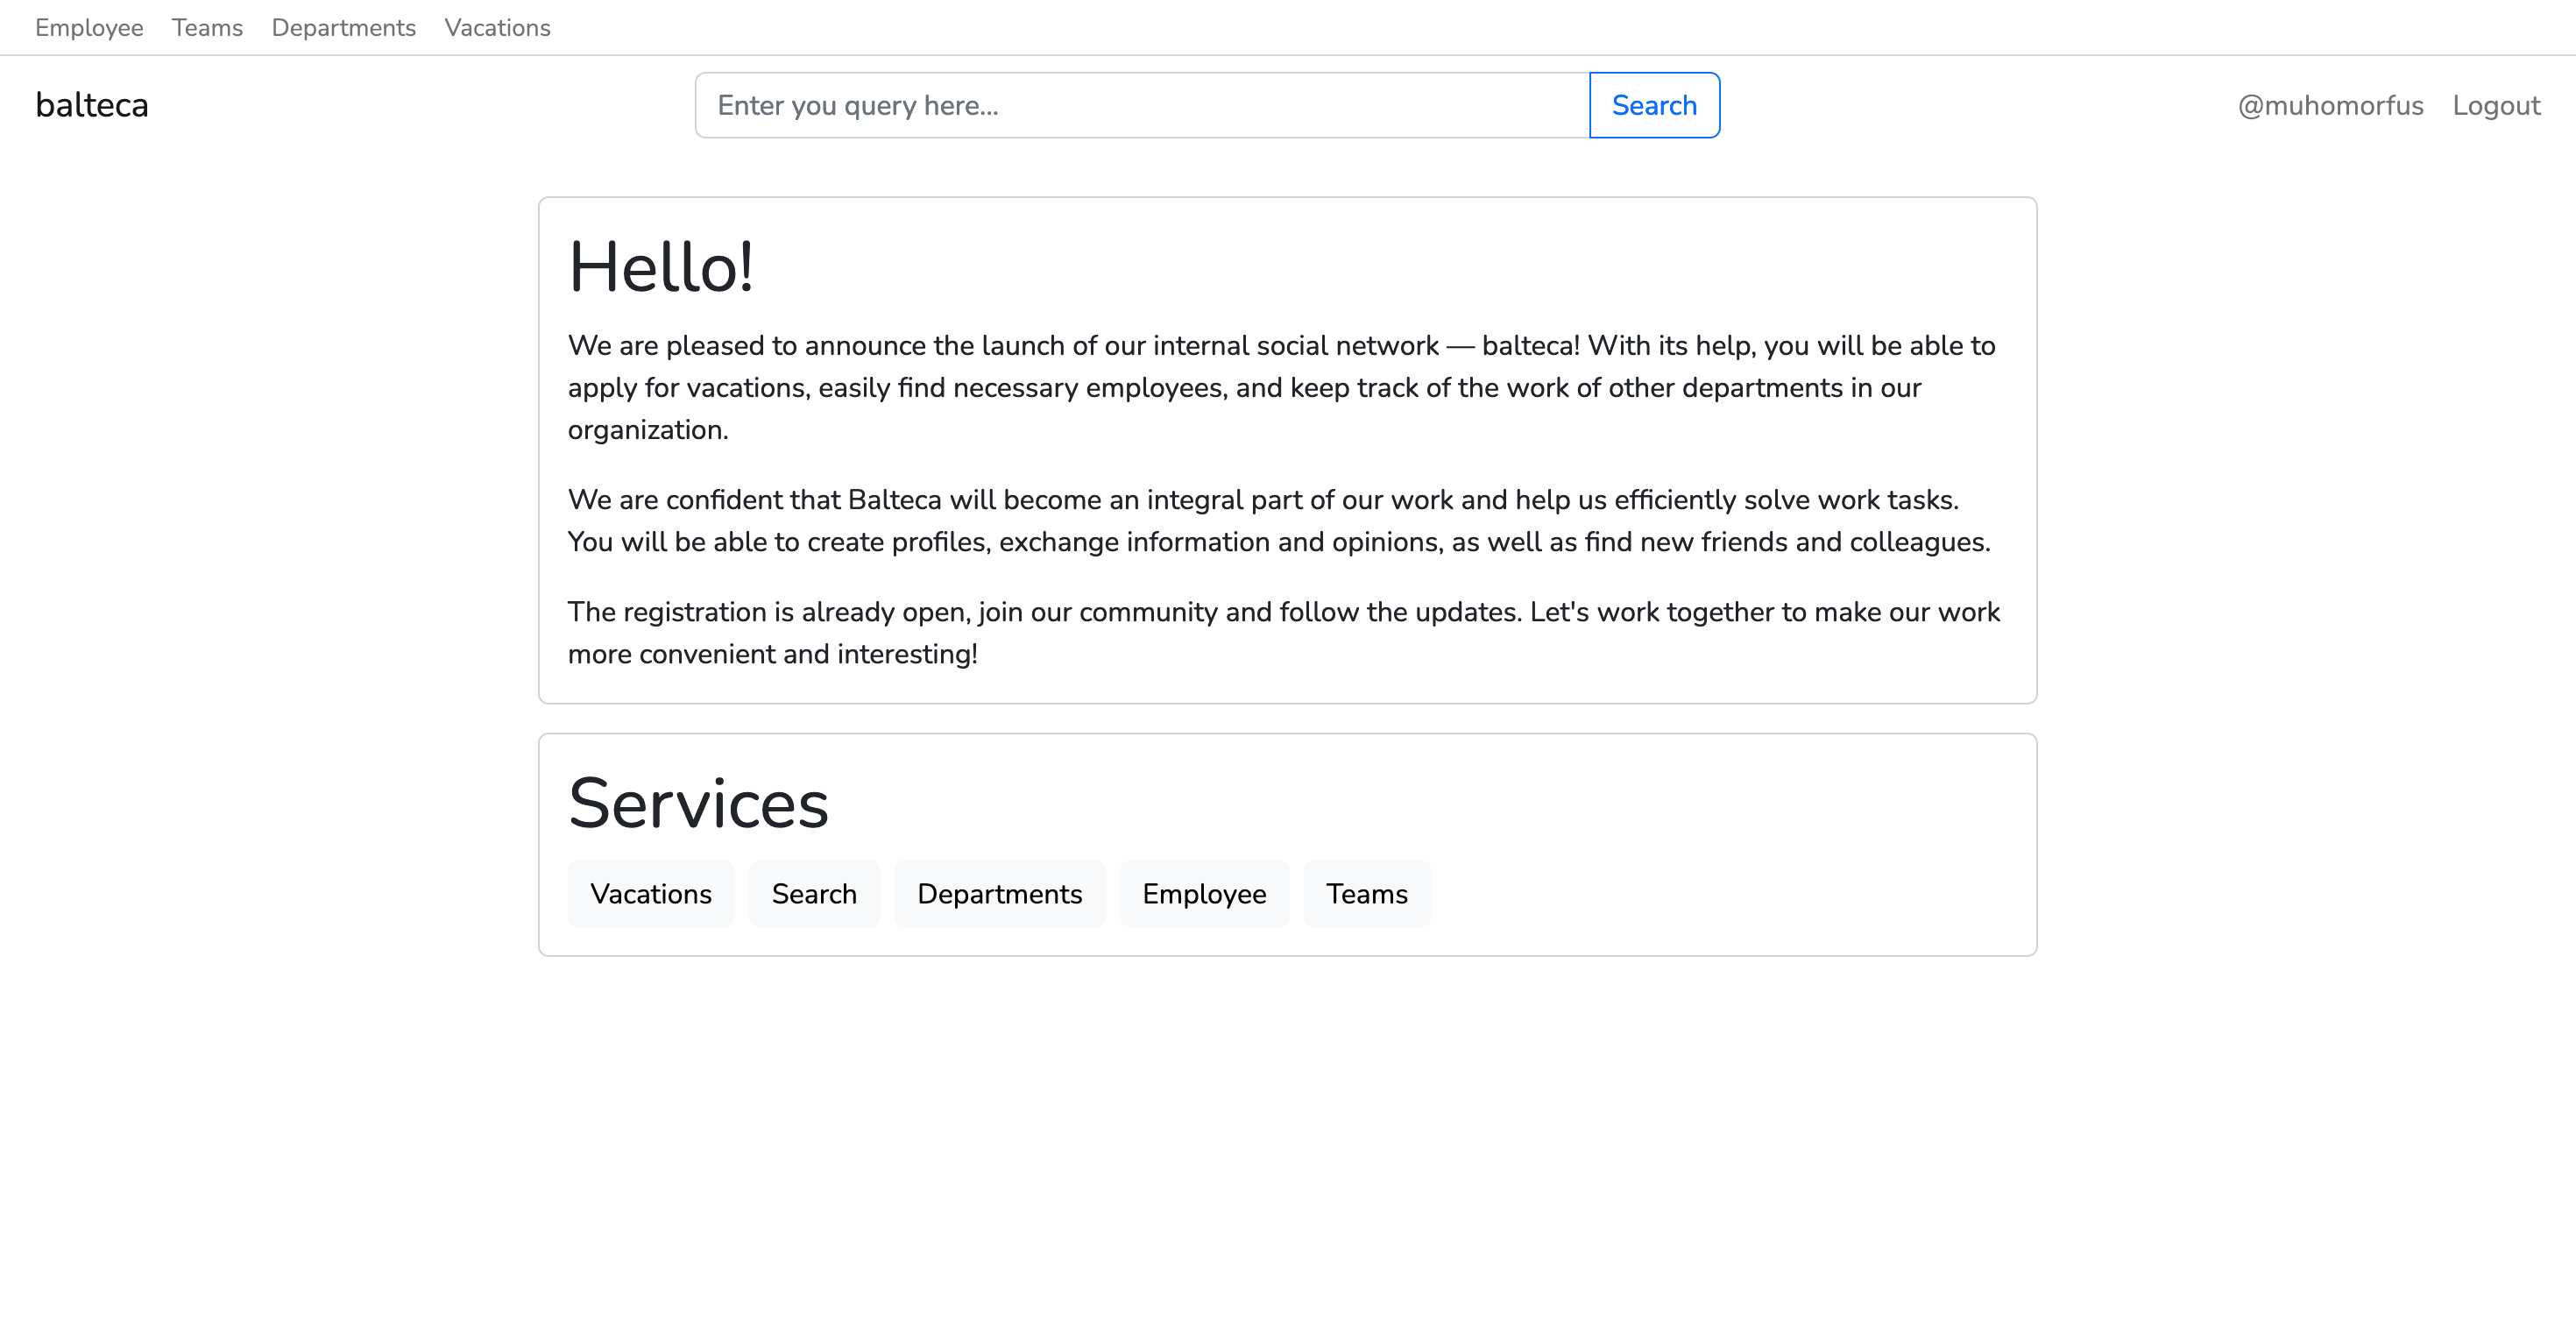
\includegraphics[width=0.9\linewidth]{assets/ss1.png}
    \caption{Главная страница}
    \label{img:ss1}	
\end{figure}

\newpage

На рис.~\ref{img:ss2} изображена страница отображения профиля пользователя.

\begin{figure}[h!]
\centering
    \includegraphics[width=0.9\linewidth]{assets/ss2.png}
    \caption{Страница профиля}
    \label{img:ss2}	
\end{figure}

На рис.~\ref{img:ss3} изображена страница результатов поиска. Поисковая строка находится в меню навигации сверху, и доступно с любой страницы.

\begin{figure}[h!]
\centering
    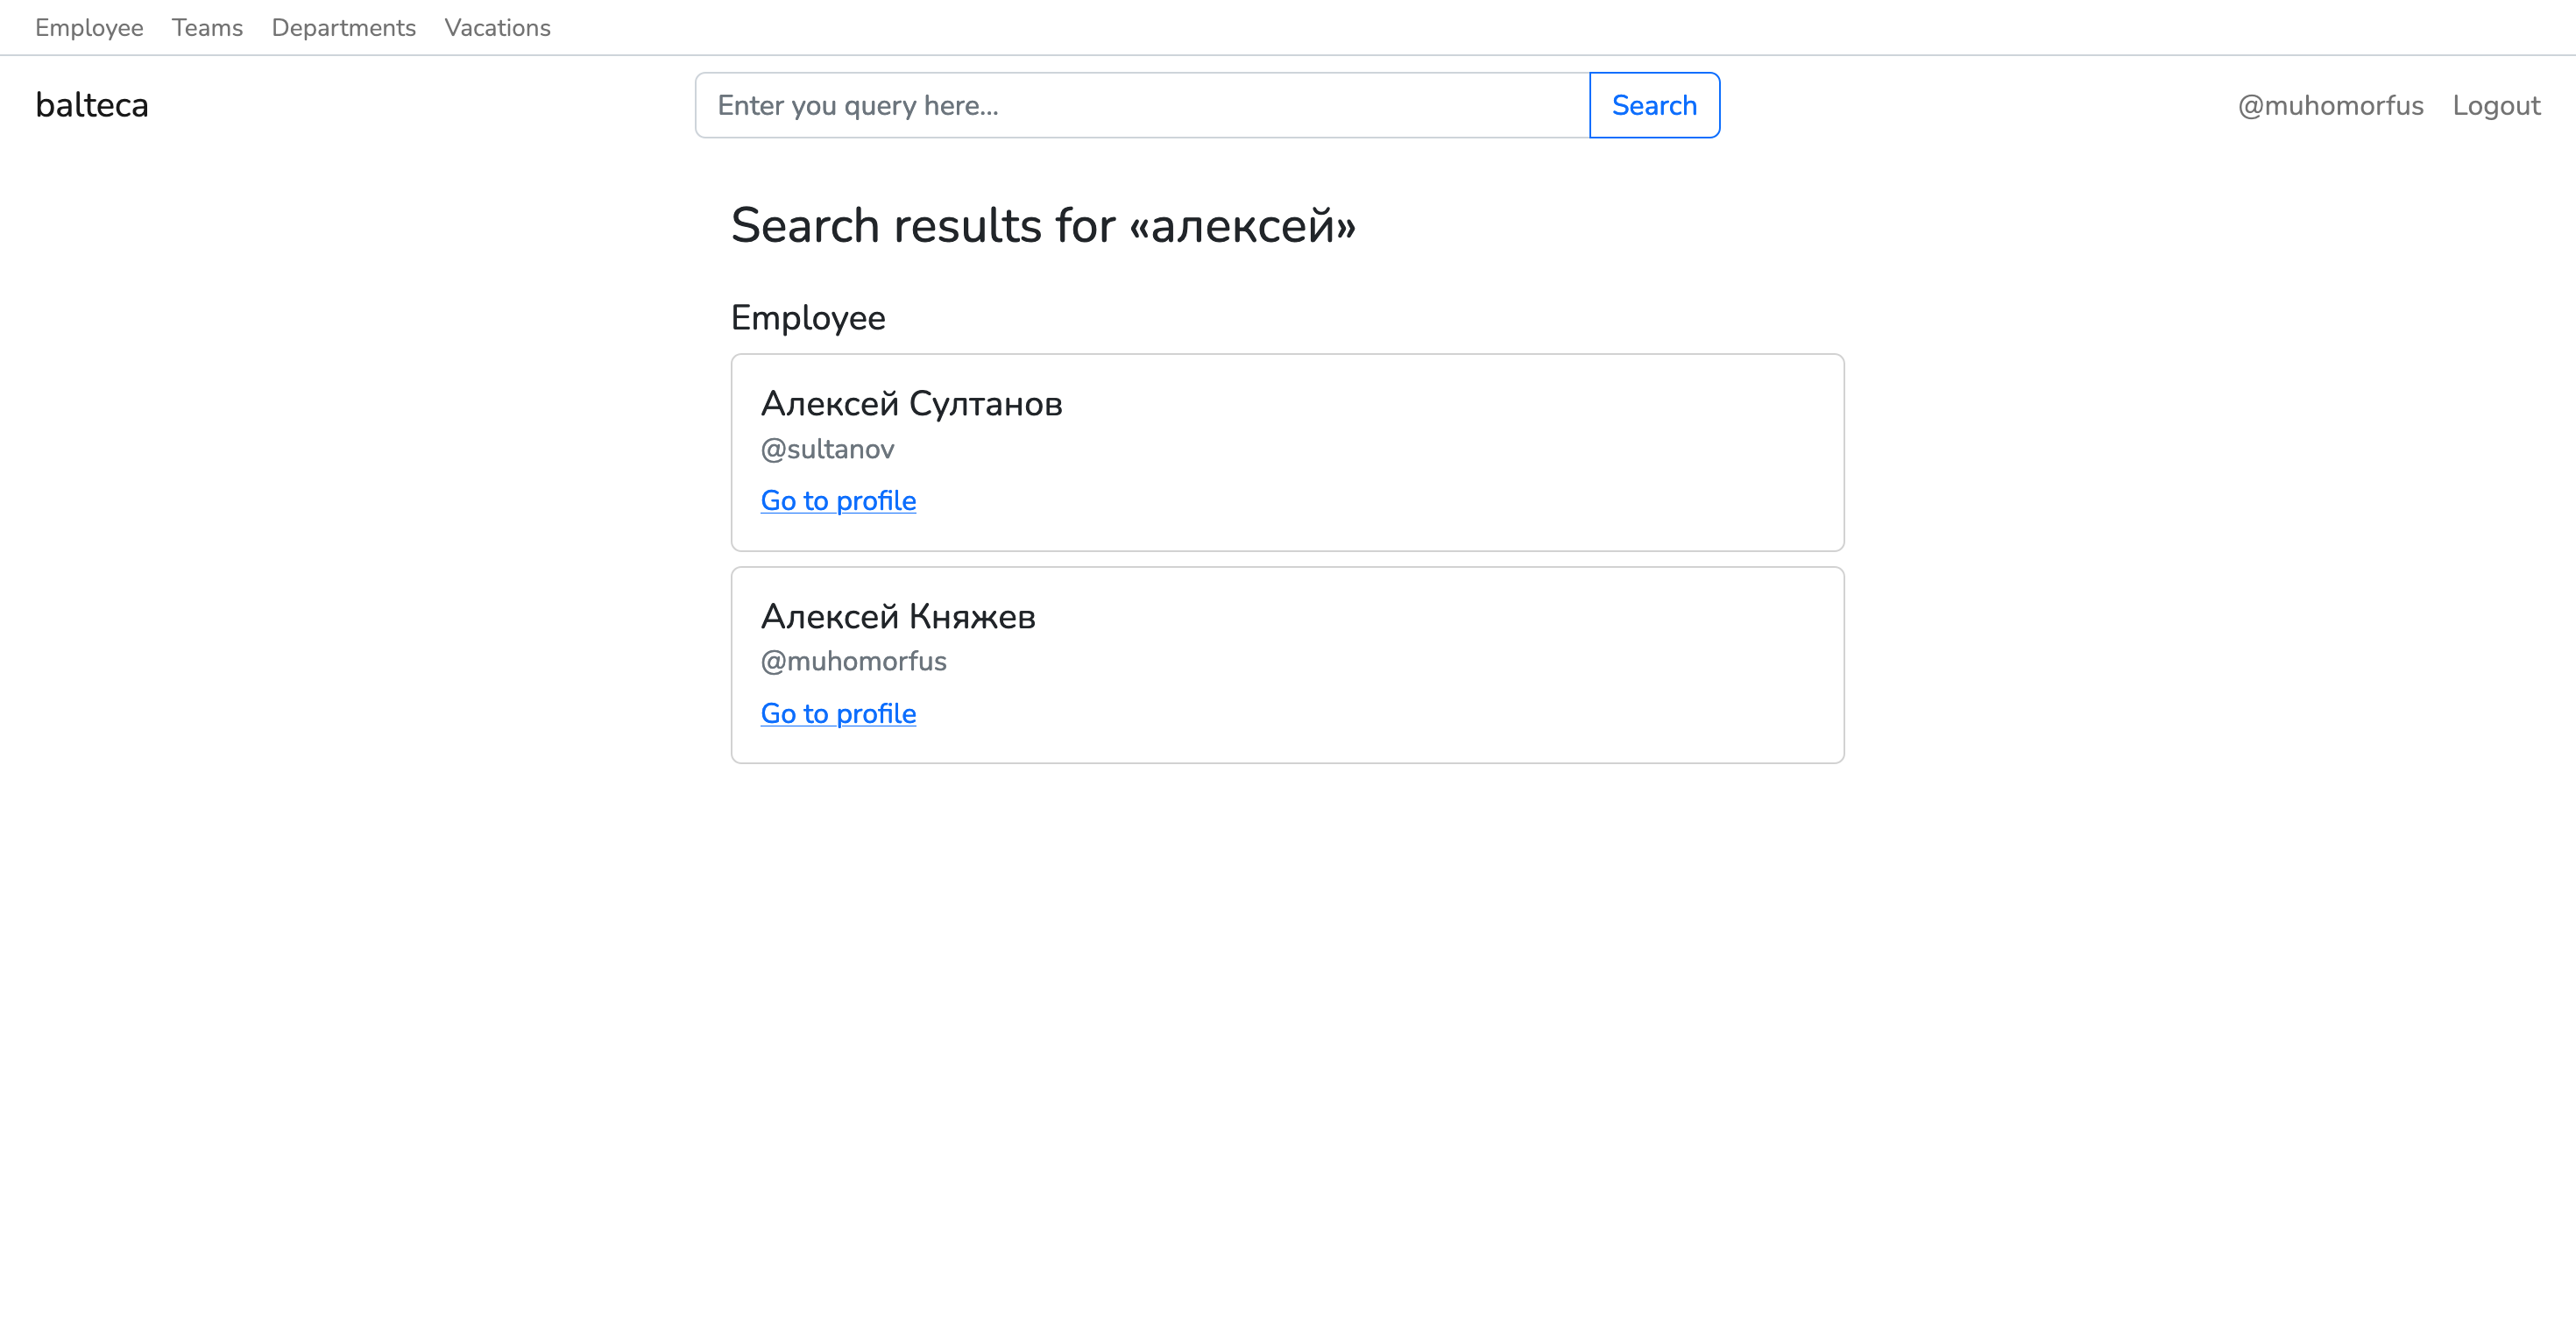
\includegraphics[width=0.9\linewidth]{assets/ss4.png}
    \caption{Страница результатов поиска}
    \label{img:ss3}	
\end{figure}

